\documentclass[a4paper]{article}

%% Language and font encodings
\usepackage[english]{babel}
\usepackage[utf8x]{inputenc}
\usepackage[T1]{fontenc}

%% Sets page size and margins
\usepackage[a4paper,top=3cm,bottom=2cm,left=3cm,right=3cm,marginparwidth=1.75cm]{geometry}

%% Useful packages
\usepackage{amsmath}
\usepackage{amssymb}
\usepackage{graphicx}
\usepackage[colorinlistoftodos]{todonotes}
\usepackage[colorlinks=true, allcolors=blue]{hyperref}
\usepackage{times}
\usepackage{url}
\usepackage{latexsym}
\usepackage{natbib}
\usepackage{graphicx}
\usepackage{paralist}
\graphicspath{ {figs/} }


%% \usepackage[numbers]{natbib}

\title{Learning Representations of Semantic Role Fillers in Events with Neural Networks}
\author{Author: Xudong Hong \\ 
Supervisor: Asad Sayeed, Vera Demberg}

\begin{document}
\maketitle

\begin{abstract}
We introduce a neural network model capturing both lexical and semantic features of event participants. Possible methods to composite word and semantic role representations are discussed. Making use of tensor factorisation on role-specific word embedding \citep{tilk-EtAl:2016:EMNLP2016}, we represent the order-3 tensor feature space using 3 matrices. Then we add non-linearity and construct the model as a neural network. The model is trained in multitask style to counter both semantic role-filler prediction and semantic role-label prediction tasks. Comparing to previous works, the model has improvement on both semantic role/role-filler modelling and human thematic fit judgement correlations task. Moreover, the trained model has high accuracy on semantic role prediction. 
\end{abstract}



\section{Introduction}
Event participants can be mapped to arguments of a predicate.
A level of representation to show the common characteristics is \textit{semantic roles} which express the abstract role of the argument of a predicate can taken in an event. 
For example, 
\begin{figure}[ht]
\centering
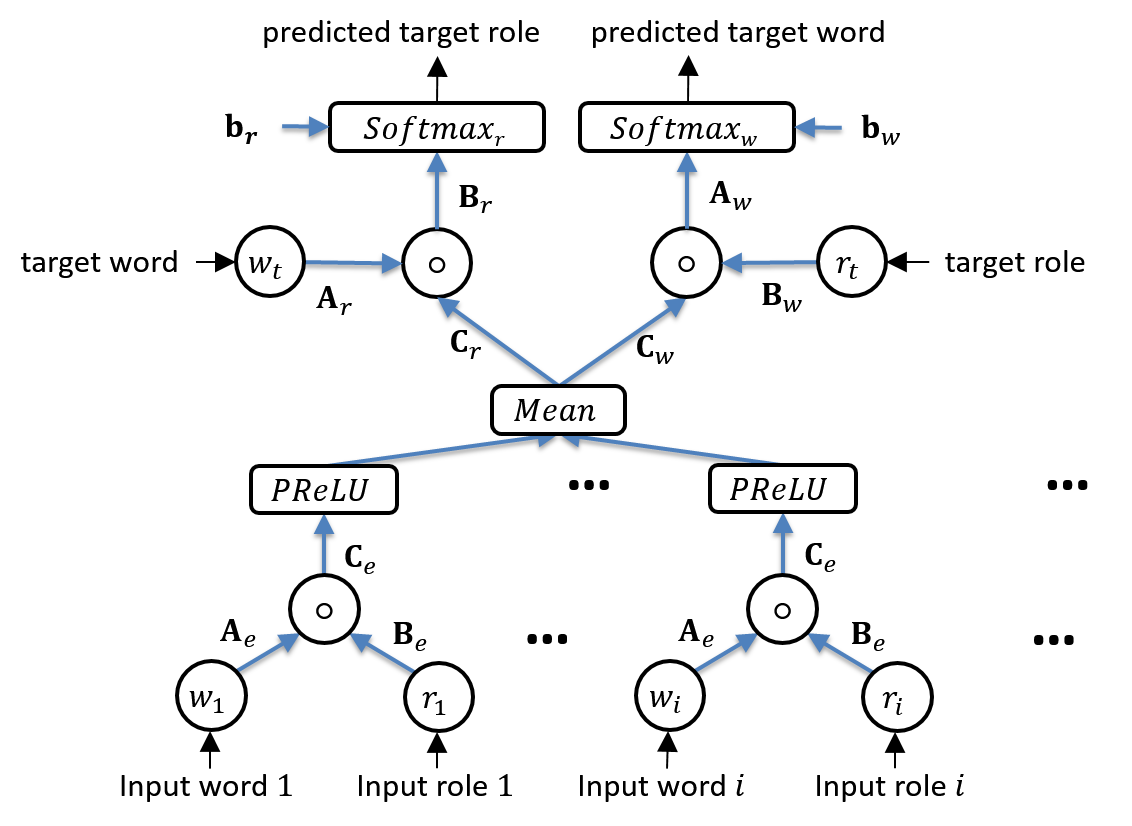
\includegraphics[width=0.8\textwidth]{BOP.png}
\caption{\label{fig:SemanticRoles} An event with predicate and event participants. Each event participant is annotated with its corresponding semantic role}
\end{figure}

\noindent


\noindent
Distributed representation of words is useful in natural language understanding, natural language generation and machine translation. There are many efforts on learning word embedding from large scale text corpora. Nevertheless for generality, most of these works only use raw word as input without using any semantic features. 


\noindent
The semantic role labeling task is to assign semantic role labels to the event participants in an event. After many years of research, pre-trained semantic role labeling systems are quite reliable. However, most of these works only assign labels to the whole constituents or phrases. \citet{Sayeed2014} proposed an unsupervised method of assigning semantic roles to headwords in event participants to construct a corpus. The raw text are firstly processed by a state-of-the-art semantic role labeller SENNA \citep{Collobert}. Then a dependency parser Malt Parser is used to extract the headwords of the event participants together with some heuristics.


\noindent
In this paper, we present a model ...



\section{Related Works}

\subsection{Representation Learning}

Words can be represented with vectors in adjacent matrix using count based method. But when it comes to the practice, this kind of method has a problem of sparsity. The vector of count-based method is discrete, high-dimensional and sparse. Distributed representation is an effective method to tackle sparsity of high-dimensional vectors. \\
\noindent
\citet{mikolov2013distributed} proposed recurrent neural network based language model.

\subsection{Semantic Role Labeling}
There are many state-of-the-art SRL systems \citep{collobert2011natural, titov2011bayesian}. \citet{roth2016neural} proposed PathLSTM which made use of syntactic features. But \citet{marcheggiani2017simple} claimed that syntactic features is not necessary for semantic role labeling.

\subsection{Cognitive Modelling}
\subsubsection{Event Level Model}
Event-level knowledge does affect human expectations for verbal arguments \citep{baroni2010distributional}. \\
\noindent 
Regarding to models of events, \citet{tilk2016event} proposed two models: \textit{non-incremental model} and \textit{incremental model}. For the \textit{non-incremental model}, they simply summed all the vectors $p$ of event participants together to represent the event $e$ as a vector:
\begin{equation} \label{eq:20}
\begin{aligned}
    \mathbf{e}
        &= \sum_{l=1}^{L} \mathbf{p}_{l} \\
\end{aligned}
\end{equation}
where $L$ is the number of participants in event $e$. \\
\noindent
When it comes to the \textit{incremental model}, they added a recurrent unit to express participant order not only within event but also across different events. Moreover, a binary indicator $b$ is used to detect the event boundaries. $b$ equals to $1$ if the target word belongs to current event, otherwise $0$. So the event representation vector is: 
\begin{equation} \label{eq:21}
\begin{aligned}
    \mathbf{e}
        &= \mathbf{p} + \mathbf{h_{t-1}}\mathbf{W}_h + b\mathbf{v}
\end{aligned}
\end{equation} 
where $\mathbf{v}$ is the parameter vector of event boundary. $\mathbf{h_{t-1}}$ is the hidden vector of last time step in the recurrent unit. $\mathbf{W}_h$ is the parameter matrix of recurrent unit. 

\subsubsection{Thematic Fit Evaluation}
\citet{sayeed2014combining} 
Extract thematic features using semantic role labeler SENNA \citep{collobert2011natural}.
Construct distributional memory model. 



\section{Representation of Event Participants}
\subsection{Event Participant Embedding}
We intend to learn meaningful representation in semantic space of words and roles. Firstly we define the symbolic representation for words. Word $a_i$ is encoded as one-hot row vector $\mathbf{w}_i = [00...1...0]$ containing exactly one $1$ value in the position of word index $i$ and other values are all $0$, where $|\mathbf{w}_i| = |V|$ and $V$ is the word vocabulary. In this vector space, words are mutual exclusive to each other.  \\
\noindent
Futher than that, we need to obtain a distributed representation that is smoother. So we compute the inner product between $\mathbf{w}_i$ and a embedding matrix $\mathbf{A} \in \mathbb{R}^{|V| \times k}$ as $\mathbf{A}_{(i)} = \mathbf{w}_i \mathbf{A}$. The vector $\mathbf{w}_i$ is now mapped to low-dimensional vector $\mathbf{A}_{(i)} \in \mathbb{R}^k$ which is the $i$-th row of matrix $\mathbf{A}$. The symbolic representations of words are transformed into distributed representations. \\
\noindent
In addition to word embedding, we want to learn the representation of words given a specific semantic role. Performing matricization on a order-3 tensor which contains word-role-word tuple onto a matrix can obtain vectors from different semantic spaces \citep{baroni2010distributional}. Inspiring by this idea, we add one more dimension of semantic role to the word embedding matrix and obtain a third-order tensor $\mathbf{T} \in \mathbb{R}^{|V| \times |R| \times d}$. For each word $\mathbf{w}_i$ and each semantic role $\mathbf{r}_j$, there is a corresponding vector $\mathbf{T}_{(ij)}$ with length of $d$ where $i \in [1, |V|]$ and $j \in [1, |R|]$. This vector is named as \textit{role-specific word embedding} vector \citep{tilk2016event} which can be further simplified to \textbf{event participant embedding} vector.



\section{Some examples to get started}

\subsection{How to include Figures}

First you have to upload the image file from your computer using the upload link the project menu. Then use the includegraphics command to include it in your document. Use the figure environment and the caption command to add a number and a caption to your figure. See the code for Figure \ref{fig:frog} in this section for an example.

\begin{figure}
\centering
\includegraphics[width=0.3\textwidth]{frog.jpg}
\caption{\label{fig:frog}This frog was uploaded via the project menu.}
\end{figure}

\subsection{How to add Comments}

Comments can be added to your project by clicking on the comment icon in the toolbar above. % * <john.hammersley@gmail.com> 2016-07-03T09:54:16.211Z:
%
% Here's an example comment!
%
To reply to a comment, simply click the reply button in the lower right corner of the comment, and you can close them when you're done.

Comments can also be added to the margins of the compiled PDF using the todo command\todo{Here's a comment in the margin!}, as shown in the example on the right. You can also add inline comments:

\todo[inline, color=green!40]{This is an inline comment.}

\subsection{How to add Tables}

Use the table and tabular commands for basic tables --- see Table~\ref{tab:widgets}, for example. 

\begin{table}
\centering
\begin{tabular}{l|r}
Item & Quantity \\\hline
Widgets & 42 \\
Gadgets & 13
\end{tabular}
\caption{\label{tab:widgets}An example table.}
\end{table}

\subsection{How to write Mathematics}

\LaTeX{} is great at typesetting mathematics. Let $X_1, X_2, \ldots, X_n$ be a sequence of independent and identically distributed random variables with $\text{E}[X_i] = \mu$ and $\text{Var}[X_i] = \sigma^2 < \infty$, and let
\[S_n = \frac{X_1 + X_2 + \cdots + X_n}{n}
      = \frac{1}{n}\sum_{i}^{n} X_i\]
denote their mean. Then as $n$ approaches infinity, the random variables $\sqrt{n}(S_n - \mu)$ converge in distribution to a normal $\mathcal{N}(0, \sigma^2)$.


\subsection{How to create Sections and Subsections}

Use section and subsections to organize your document. Simply use the section and subsection buttons in the toolbar to create them, and we'll handle all the formatting and numbering automatically.

\subsection{How to add Lists}

You can make lists with automatic numbering \dots

\begin{enumerate}
\item Like this,
\item and like this.
\end{enumerate}
\dots or bullet points \dots
\begin{itemize}
\item Like this,
\item and like this.
\end{itemize}

\subsection{How to add Citations and a References List}

You can upload a \verb|.bib| file containing your BibTeX entries, created with JabRef; or import your \href{https://www.overleaf.com/blog/184}{Mendeley}, CiteULike or Zotero library as a \verb|.bib| file. You can then cite entries from it, like this: \cite{greenwade93}. Just remember to specify a bibliography style, as well as the filename of the \verb|.bib|.

You can find a \href{https://www.overleaf.com/help/97-how-to-include-a-bibliography-using-bibtex}{video tutorial here} to learn more about BibTeX.

We hope you find Overleaf useful, and please let us know if you have any feedback using the help menu above --- or use the contact form at \url{https://www.overleaf.com/contact}!


\bibliographystyle{acl_natbib}
\bibliography{mtrf}


\end{document}